\chapter{Design}
Det er i projektet arbejdet lodret ned igennem lagene ved udvikling af nye features. I dette afsnit er det valgt at beskrive to features igennem lagene, for at eksemplificere selve designet af systemet. For fuld beskrivelse af systemdesignet, se dokumentationen.

\section{Modeldesign}

Ud fra domæneanalysen er data der giver mening at persistere fundet, og på fig. \ref{fig:BarteradModel} A) kan det ses hvad der fra domæneanalysen skulle gemmes i forbindelse med BarterAds.

\begin{figure}[H]
	\centering
	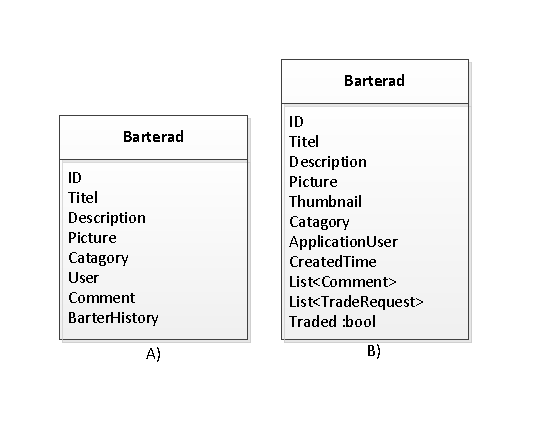
\includegraphics
	[width=140mm]{figures/BarterAdModels.pdf}
	\caption{A) BarterAd model fra domæneanalyse  B) Aktuel model}
	\label{fig:BarteradModel}
\end{figure} 

Efter arbejde, og iterationer igennem den agile arbejdsmetode er der udfærdiget et endeligt modeldesign af barterads, som kan ses på \ref{fig:BarteradModel} B.  
I designfasen blev det bestemt hvilke sikkerhedskriterier data i databasen skal overholde. Til dette konkrete eksempel er der en række krav til modellen som skal være opfyldt. Disse ses her:

\begin{itemize}
	\item Barterads skal være tilknyttet en ApplicationUser
	\item Barterads skal have et oprettelsestidspunkt, men dette laves her
	\item Barterads må have en maksiaml beskrivelseslængde på 500 tegn
\end{itemize}

Modellen opretter igennem Entity Framework databasestrukturen, og derefter tilgås dataene ved det tidligere nævnte repository pattern, der standardiserer måden at tilgå data på.


\section{Controller}  

I controllerne ligger selve funktionaliteten af BargainBarter system. Det er controllernes opgave at opdatere det view, som brugeren ser, samt styre kommunikationen mellem viewet og modellen. \\
 
\subsection{Opret annonce}
\noindent Som det ses på figur \ref{fig:SDOpretBarterAd} trykker brugeren ind for at lave en ny annonce. Systemmet registrerer at der er trykket på en knap, og kalder den til view elementets tilhørende action. Igennem denne action returneres \textit{Create BarterAd} viewet. I dette view kan der indtastes data til BarterAds. Brugeren indtaster data og submitter og controlleren opretter så selve BarterAd'en. I oprettelsen genereres tilhørsbrugeren og oprettelsestidspunkt. \\


\begin{figure}[H]
	\centering
	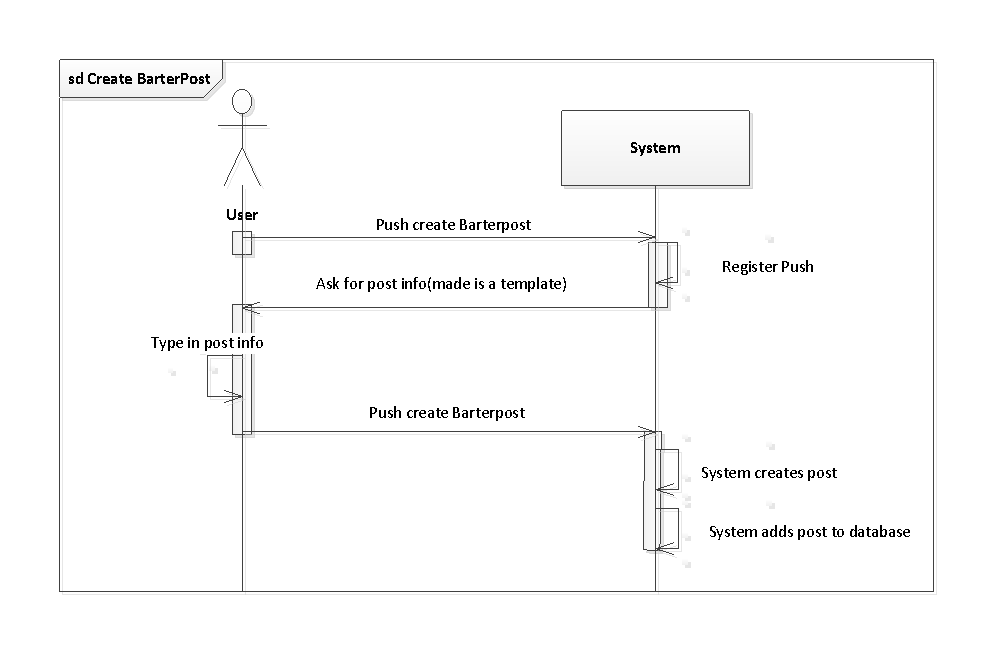
\includegraphics
	[width=140mm]{../Dokumentation/figures/SDOpretBytteAnnonce.PDF}
	\caption{Sekvensdiagram for oprettelse af barterads}
	\label{fig:SDOpretBarterAd}
\end{figure}

Den tidligere beskrivelse af anonnceoprettelse er en happy path beskrivelse, som ikke tager højde for fejl. I design og implementering af alle controllers skal der holdes styr på mulige fejl. For eksempel er der i oprettelsen sikret at brugeren skal være logget ind. Dette holder controlleren styr på. Desuden tjekker viewet og modellen at alle datafelter er udfyldte, og fortæller brugeren hvad de mangler at udfylde.

\subsection{Søgning}     











